%-----------------------------------------------------------------
% POSTER CONTENTS
% !TEX root = ../main.tex
%-----------------------------------------------------------------

%-----------------------------------------------------------------
\begin{block}{\vspace*{1.6cm}}
% \begin{block}{Data shows}
	\begin{figure}[H]
		\centering
		\subfloat[Marginal distribution of the $PDI$]{%
			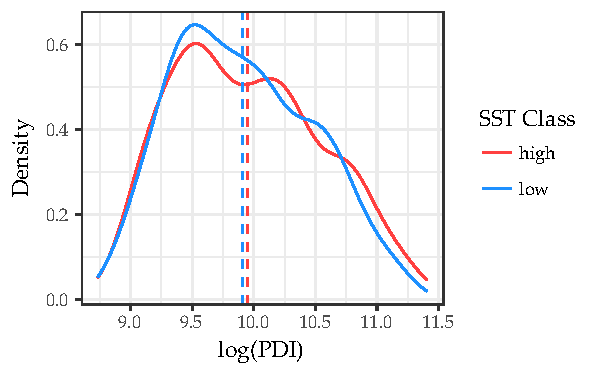
\includegraphics[width=0.5\textwidth]{./images/natl-marginals-pdi}
			\label{fig:natl-marginals-pdi}%
			}%
		\subfloat[Marginal distribution of the lifetime]{%
			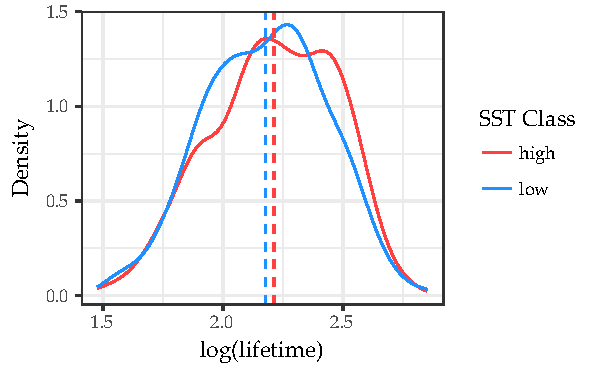
\includegraphics[width=0.5\textwidth]{./images/natl-marginals-lifetime}
			\label{fig:natl-marginals-lifetime}%
			}%
		\caption{Marginal analysis for the variables of the bivariate lognormal distribution for the North Atlantic basin data}
		\label{fig:natl-marginals}
	\end{figure}

	It is important to notice that the relationships between the TC variables are of non-linear nature. This naturally means that our regressions need to follow a so-called log--log model:
	\begin{equation}\label{eq:lm-model-bis}
		\log \Psi = \alpha + \beta \log \Phi + \epsilon ,
	\end{equation}
	where $\log \Psi \equiv Y$ and $\log \Phi \equiv X$.

\end{block}

\begin{block}{Methodology}
% 	%\begin{multicols}{2}
% 	Instead of working with the exact joint
% 	%bivariate log-normal
% 	distributions $f$, we study the expected value of the distributions:
% 	\begin{equation}
% 		E(Y \mid X = x )_{\text{low}} = E(Y \mid X = x )_{\text{high}},
% 	\end{equation}
% 	where $E(Y \mid X = x )$ is estimated by performing a ordinary least squares (OLS) regression analysis on the data sets.

% 	\medskip
% 	It is important to notice that the relationships between the TC variables are of non-linear nature. This naturally means that our regressions need to follow a so-called log--log model:
% 	\begin{equation}\label{eq:lm-model-bis}
% 		\log \Psi = \alpha + \beta \log \Phi + \epsilon ,
% 	\end{equation}
% 	where $\log \Psi \equiv Y$ and $\log \Phi \equiv X$.
% 	% \medskip
% 	%\end{multicols}
% \end{block}

% \vspace*{-1cm}
% \begin{block}{}
	%\begin{multicols}{2}
	In essence, our methodology will consist in comparing the low-SST and high-SST regression models using non-parametric permutation tests.

	\medskip
	For the permutation tests, we use bootstrap %and
	\nocite{Analysis2003} %the bootstrap-$t$ method
	in order to get a more robust estimation of the value of the different studied statistical coefficients (such as $\hat{\beta}_{0}$, $\hat{\beta}_{1}$, $R^{2}$) and their standard errors than the one obtained using the value obtained using the OLS method. Withal, we compare the results obtained using both methods.

	% We compare the results obtained using (a) the OLS method, and (b) the bootstrap-$t$ method
	%\end{multicols}
\end{block}

%-----------------------------------------------------------------
\begin{block}{}
% \begin{block}{\vspace*{1.72cm}}
	% We use bootstrap and the bootstrap-$t$ method in order to get a better estimation of the value of the different studied statistical coefficients (such as $\hat{\alpha}$, $\hat{\beta}$, $r^{2}$) and their standard errors than the one obtained using the value obtained using the OLS method.

	The following null hypothesis is proposed to test the data:
	\begin{equation}
		H_{0} : \hat{\beta}_{0,h} = \hat{\beta}_{0,l} \wedge \hat{\beta}_{1,h} = \hat{\beta}_{1,l}
		.
	\end{equation}

	We use the following statistics:
	\begin{equation}
		T^{(1)} = \abs{\hat{\beta}_{0,h} - \hat{\beta}_{0,l}}
		\qc
		T^{(2)} = \abs{\hat{\beta}_{1,h} - \hat{\beta}_{1,l}}
		\qc
		T^{(3)} = \abs{ R^{2}_{h} - R^{2}_{l} } \label{eq:h0-stat-simple} .
	\end{equation}

	\citeauthor{Polko-Zajac2016} \cite{Polko-Zajac2016} proposes alternative statistics that not only consider the nominal value of the coefficient estimates, but take into account their standard errors as well:
	\begin{equation}
		T^{(4)} = \frac{\abs{\hat{\beta}_{0,h} - \hat{\beta}_{0,l}}}{\se{\hat{\beta}_{0,h} - \hat{\beta}_{0,l}}}
		\qc
		T^{(5)} = \frac{\abs{\hat{\beta}_{1,h} - \hat{\beta}_{1,l}}}{\se{\hat{\beta}_{1,h} - \hat{\beta}_{1,l}}}
		\qc
		T^{(6)} = T^{(4)} + T^{(5)} \label{eq:h0-stat-polko}.
	\end{equation}

	% where $\se{\hat{\beta}_{0,h} - \hat{\beta}_{0,l}} = \sqrt{\se{\hat{\beta}_{0,h}}^{2} + \se{\hat{\beta}_{0,l}}^{2}}$ and $\se{\hat{\beta}_{1,h} - \hat{\beta}_{1,l}} = \sqrt{\se{\hat{\beta}_{1,h}}^{2} + \se{\hat{\beta}_{1,l}}^{2}}$.
	% \begin{equation}
	% 	\se{\hat{\alpha}_{h} - \hat{\alpha}_{l}} = \sqrt{\se{\hat{\alpha}_{h}}^{2} + \se{\hat{\alpha}_{l}}^{2}}
	% 	\qc
	% 	\se{\hat{\beta}_{h} - \hat{\beta}_{l}} = \sqrt{\se{\hat{\beta}_{h}}^{2} + \se{\hat{\beta}_{l}}^{2}}
	% \end{equation}
\end{block}

\vspace*{0.75cm}
\begin{block}{Results}
	%\begin{multicols}{2}
	% Our empirical results show a remarkable correlation in the joint distribution of lifetime and wind speed, as seen in \Cref{fig:regression}.

	% \begin{block}{ }
	% 	\begin{figure}
	% 		\vspace*{-1.1cm}
	% 		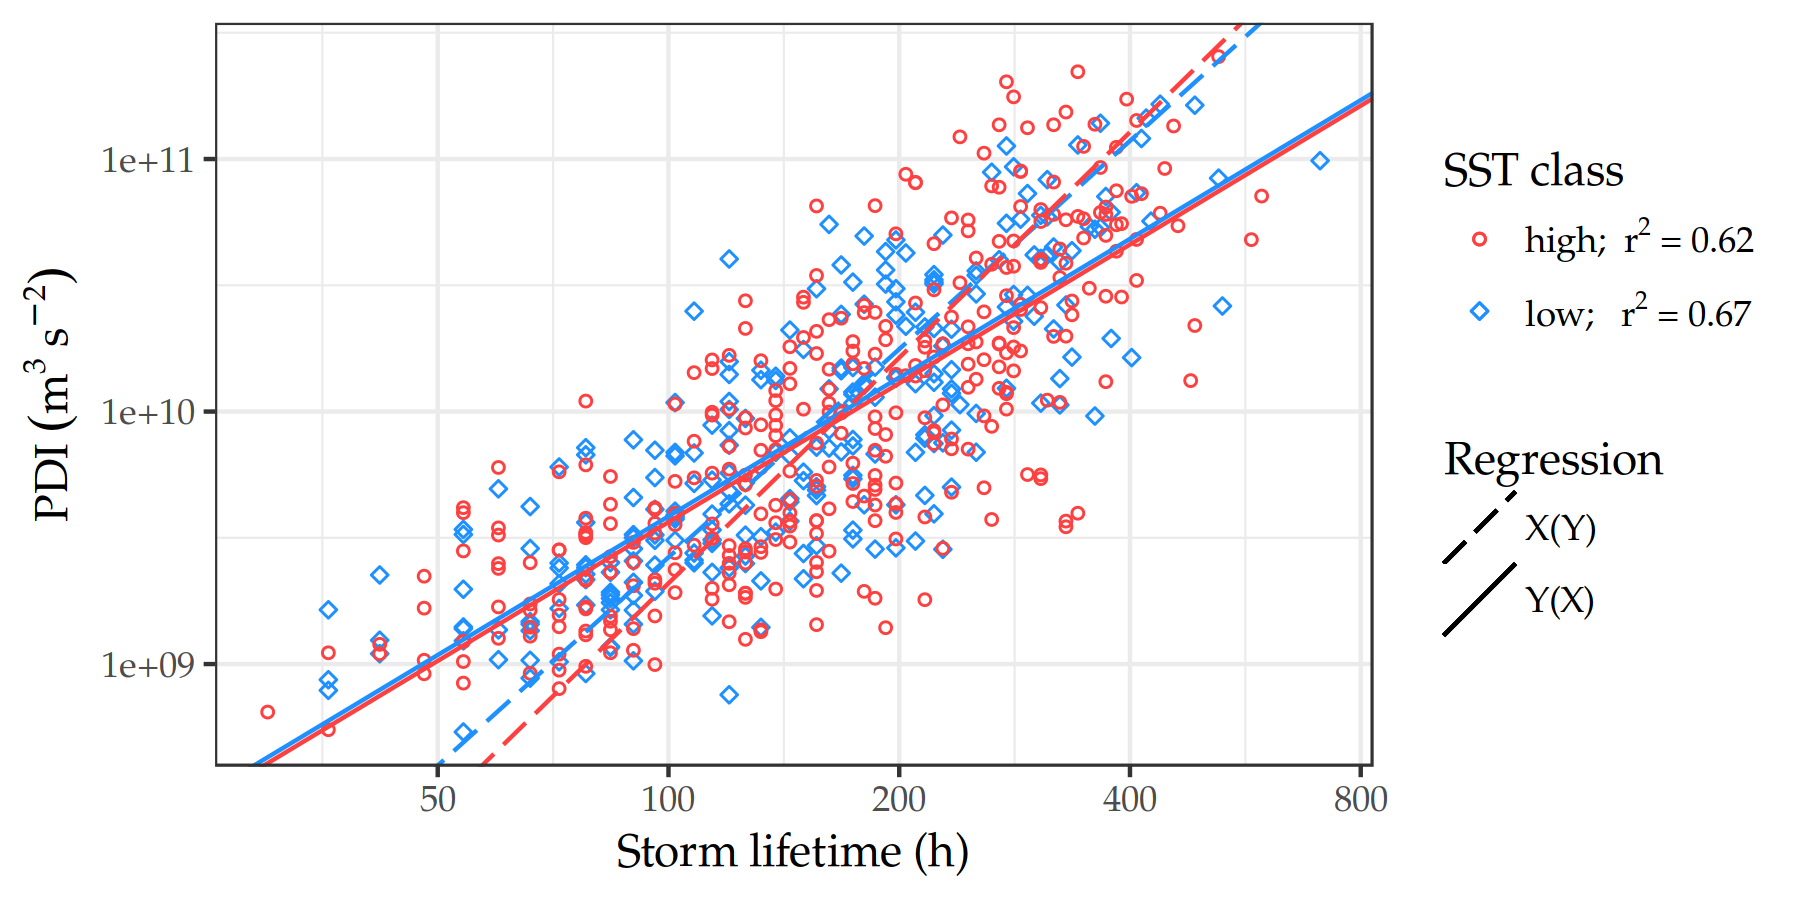
\includegraphics[width=0.95\linewidth]{images/scatter_natl.png}
	% 		\caption{~$PDI$ vs lifetime regression analysis for tropical-cyclones (excluding tropical depressions) on the North Atlantic basin}
	% 		\label{fig:regression}
	% 	\end{figure}
	% \end{block}

	%\end{multicols}
% \end{block}

% \begin{block}{}
	The value of the studied statistics $T^{(i)}$ obtained from the N.~Atl. data set can be seen in \Cref{tab:perm-natl-ols-T}.
	\begin{table}[H]
		\centering
		\begin{tabular}{cccccccc}
		\toprule
		\toprule
		$X$   & $Y$   & $T^{(1)}$ & $T^{(2)}$ & $T^{(3)}$ & $T^{(4)}$ & $T^{(5)}$ & $T^{(6)}$ \\
		\midrule
		lifetime & $PDI$ & $0.289$ & $0.027$ & $0.048$ & $1.404$ & $1.324$ & $2.727$ \\
		$PDI$ & lifetime & $0.007$ & $0.007$ & $0.054$ & $0.031$ & $0.065$ & $0.095$ \\
		\bottomrule
		\end{tabular}
		\caption{~Value of the studied statistics for North Atlantic basin data set}
		\label{tab:perm-natl-ols-T}
	\end{table}

	The results of the permutation tests performed on the N.~Atl. data can be seen in \Cref{tab:perm-natl-boot-p-vals}.
	% \begin{table}[H]
	% 	\centering
	% 	\begin{tabular}{cccccccc}
	% 	\toprule
	% 	\toprule
	% 	$X$  & $Y$       & $T^{(1)}$ & $T^{(2)}$ & $T^{(3)}$ & $T^{(4)}$ & $T^{(5)}$ & $T^{(6)}$ \\
	% 	\midrule
	% 	% PDI & lifetime & $0.164$ & $0.184$ & $0.749$ & $0.160$ & $0.187$ & $0.173$ \\
	% 	PDI & lifetime & $0.176$   & $0.154$   & $0.740$   & $0.174$   & $0.148$   & $0.162$   \\
	% 	% lifetime & PDI & $0.901$ & $0.991$ & $0.750$ & $0.900$ & $0.992$ & $0.968$ \\
	% 	lifetime & PDI & $0.990$   & $0.930$   & $0.766$   & $0.990$   & $0.926$   & $0.972$   \\
	% 	\bottomrule
	% 	\end{tabular}
	% 	\caption{List of $p$-values of the standard (OLS) permutation test for the North Atlantic basin data}
	% 	\label{tab:perm-natl-ols-p-vals}
	% \end{table}

	\begin{table}[H]
		\centering
		\begin{tabular}{cccccccc}
		\toprule
		\toprule
		$X$  & $Y$       & $T^{(1)}$ & $T^{(2)}$ & $T^{(3)}$ & $T^{(4)}$ & $T^{(5)}$ & $T^{(6)}$ \\
		\midrule
		lifetime & $PDI$ & $0.146$   & $0.121$   & $0.711$   & $0.137$   & $0.117$   & $0.128$   \\
		$PDI$ & lifetime & $0.870$   & $0.806$   & $0.705$   & $0.864$   & $0.795$   & $0.830$   \\
		\bottomrule
		\end{tabular}
		\caption{List of $p$-values of the bootstrap-powered permutation test for the North Atlantic basin data}
		\label{tab:perm-natl-boot-p-vals}
	\end{table}

% \end{block}

% \begin{block}{}
	%\begin{multicols}{2}
	\vspace*{0.08cm}
	The results show that none of the performed permutation tests is able to reject the null hypothesis $H_{0}$.
	% The results suggest the following things:
	% \begin{itemize}
	% 	\item None of the performed permutation tests is able to reject the null hypothesis $H_{0}$.
	% 	\item Taking into account the standard error does not change the $p$-value significantly.% ($T^{(1)} \sim T^{(4)}$, $T^{(2)} \sim T^{(5)}$).
	% 	% \item The statistic $T^{(6)}$ is the arithmetic mean of $T^{(4)}$ and $T^{(5)}$.
	% 	\item The bootstrap-powered method does not give a significantly different result than using the standard OLS method, although it is more sensible method to hypothesis testing.
	% \end{itemize}
	%\end{multicols}
\end{block}

%-----------------------------------------------------------------
% \vspace*{0.68cm}
\begin{block}{Conclusion}
	%\begin{multicols}{2}
	% Some remarkable results can be extracted from the methodology:
	% \begin{itemize}
	% 	\item Taking into account the standard error does not change the $p$-value significantly.
	% 	\item Although the bootstrap-powered permutation test does not give a significantly different result than using the OLS-powered permutation test, it is more sensible to hypothesis testing.
	% \end{itemize}

	Our conclusions are compatible with the view of tropical cyclones as an activation process, in which, once the event has started, its intensity is kept in critical balance between attenuation and intensification (and so, higher SST does not trigger more intensification).
	%\end{multicols}
\end{block}
